%\documentclass[openany,titlepage,12pt,post]{octavo}
%foolscap,crown, post, largepost, 
%demy, medium, royal, superroyal and imperial
\documentclass[openany,titlepage,12pt]{book}
\usepackage{geometry}
\geometry{
    a5paper,
    total={67mm,137mm}%,
    %total={67mm,134mm}%,
    %left=2mm,
    %top=20mm,
}

\usepackage[utf8]{inputenc}
\usepackage{fontspec}
\usepackage{graphicx}
\graphicspath{ {./images/} }

\usepackage{fontspec}
\usepackage{lettrine}
\usepackage{Typocaps}
\usepackage{Zallman}
\usepackage{ragged2e}
\usepackage{changepage}

\usepackage[portuguese]{babel}
\usepackage{hyphenat}
\hyphenation{mate-mática recu-perar}

\usepackage{fwlw}
\usepackage{fancyhdr}
\pagestyle{fancy}
\fancyhead[CO]{\textit{\rightmark}}
\fancyhead[CE]{\textit{\leftmark}}
\fancyhead[LO]{\thepage}
\fancyhead[RE]{\thepage}
\fancyhead[LE,RO]{}
\fancyfoot[L,C]{}
\fancyfoot[R]{\usebox\NextWordBox}
\renewcommand{\headrulewidth}{0pt}
\renewcommand{\footrulewidth}{0pt}

\fancypagestyle{plain}{
  \fancyhead{}
  \fancyhead[LO,RE]{\thepage}
  \fancyfoot[C]{}%{\thepage}%
  \fancyfoot[R]{\usebox\NextWordBox}
  \renewcommand{\headrulewidth}{0pt}% Line at the header invisible
  \renewcommand{\footrulewidth}{0pt}% Line at the footer visible
}

\renewcommand{\chaptermark}[1]{\markboth{#1}{}}
\renewcommand{\sectionmark}[1]{\gdef\rightmark{#1}}
%\renewcommand{\sectionmark}[1]{\markright{\arabic{section}.\ #1}}

\usepackage{titlesec}%{}{}{0em}{\bf\LARGE}
\titleformat{\chapter}[display]
  {\normalfont\Large\centering}
  {\centering }%\thechapter}%\chaptertitlename
  {0pt}
  {}%{\Large}
\titlespacing*{\chapter} 
  {0pt}
  {6pt}
  {6pt}

\titleformat{\section}
  {\centering\normalfont
  \fontsize{13}{14} \selectfont}
  %{\thesection}
  {}{1em}{}
\titlespacing*{\section} 
   {0pt}
   {12pt}
   {12pt}
 
\titleformat{\subsection}
   {\centering\normalfont\normalsize\itshape}
   {}{1em}{}
\titlespacing*{\subsection} 
    {0pt}
    {10pt}
    {10pt}

\title{CATECISMO BRASILICO}
\author{Araújo}
\date{1686}

\newcommand{\lgS}{\char"017F}
\newcommand{\lgSS}{\char"017F\char"017F}

\usepackage{enumitem}
\setlist[enumerate]{
    leftmargin=6pt,
    topsep=3pt,
    parsep=-5pt,
    partopsep=0pt,
    itemindent=6pt
}
% \setlist[enumerate]{
%     leftmargin=12pt,
%     topsep=3pt,
%     parsep=-5pt,
%     partopsep=0pt,
%     labelsep=4pt,
%     itemindent=4pt,
%     itemsep=4pt
% }

\usepackage{etoolbox}
\newlist{alternate}{enumerate}{1}
\renewcommand\labelalternatei{\protect\ifnumodd{\value{alternatei}}{M.}{D.}}
\setlist[alternate]{
    leftmargin=6pt,
    topsep=3pt,
    parsep=-5pt,
    partopsep=0pt,
    itemindent=6pt
}
\newlist{altereven}{enumerate}{1}
\renewcommand\labelaltereveni{\protect\ifnumodd{\value{altereveni}}{D.}{M.}}
\setlist[altereven]{
    leftmargin=6pt,
    topsep=3pt,
    parsep=-5pt,
    partopsep=0pt,
    itemindent=6pt
}

\newcommand{\comecalista}[5]{
    \hspace*{-11.7pt}
    \begin{minipage}[t]{0.08\linewidth}
        \flushright #1\\#2
    \end{minipage}
    \hspace{0pt}
    \begin{minipage}[t]{0.94\linewidth}
        \lettrine
        [findent =2pt, nindent=0pt,  lines=2]
        {#3}{#4}#5
    \end{minipage}
    \vspace*{-3pt}
}

\begin{document}

\setmainfont[Ligatures=Historic, Style=Historic]
% %{Liberation Serif}%
% %{DejaVu Serif}%
{EB Garamond}
\maketitle

\begin{titlepage}
    \begin{center}
        CATECISMO
        \vspace*{15pt}

        {\huge BRASILICO}
        \vspace*{15pt}

        {\tiny DA}
        \vspace*{15pt}

        DOUTRINA CHRISTAÃ
        \vspace*{15pt}

        {\tiny PUBLICADO DE NOVO} 
        \vspace*{15pt}

        {\tiny POR}
        \vspace*{15pt}

        JULIO PLATZMANN
        \vspace*{15pt}

        {\tiny EDIÇÂO FACSIMILAR}
        \vspace*{60pt}

        {\tiny LEIPZIG
        \vspace*{15pt}

        B. G. TEUBNER
        \vspace*{15pt}

        1898}

    \end{center}  
    \clearpage
\end{titlepage}

\begin{center}
    \vspace*{20pt}
    {\huge CATECISMO}
    \vspace*{20pt}

    {\large BRASILICO}
\end{center}
\pagebreak

%começa o texto
\begin{center}
    {\large CATECISMO\\}
    \vspace*{8pt}
    {\huge BRASILICO}
    \textit{\\Da Doutrina Chri\lgS tãa,}
    \\Com o Ceremonial dos Sacramentos, \&
    \\mais actos Parochiaes.
    \textit{\\COMPOSTO}
    \\Por Padres Doutos da Companhia de
    \\JESUS,
    \textit{\\Aperfeiçoado, \& dado a luz}
    \\Pelo Padre ANTONIO DE ARAUJO
    \\da me\lgS ma Companhia,
    \textit{\\Emendado ne\lgS ta \lgS egunda impre\lgSS aõ}
    \\Pelo P.BERTHOLAMEU DE LEAM
    \\da me\lgS ma Companhia,

    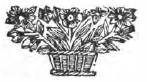
\includegraphics{img}
    \\{\huge LISBOA.}
    \\Na Officina de MIGUEL DESLANDES
    \\M. D C. L X X X V I
    \textit{\\Com todas as licenças nece\lgSS arias}

\end{center}
\clearpage
\pagebreak
%Começo do primeiro capítulo
%\vspace*{-\baselineskip}
\begin{center}
    
\includegraphics[scale=0.20]{01-poemas_brasilicos.png}
\end{center}
\unskip
\vspace*{-20pt}
{\let\clearpage\relax \chapter{POEMAS BRASILICOS}}%\chapter{POEMAS BRASILICOS}
\chaptermark{Poemas Bra\lgS ilicos}
\vspace{10pt}

\section{Do Padre Chri\lgS tovaõ Valente,\\Theologo da Companhia de JESUS,}
\sectionmark{Poemas Bra\lgS ilicos}

\subsection{Emendados para os mininis cantarem\\
ao Santi\lgSS imo nome de JESUS.}

\lettrine[findent =4pt, nindent=0pt, lines=5]
{\zall{I}}{E}SU, moropyçyroána,\\
JESU, tecó catú iâra,\\
JESU, toryberecoára,\\
JESU, xe poçánga ymána\\
JESU, xe remimotára.

Päí JESU, xepoçánga,\\
Xe pyá, xe recobé,\\
Xe pëá umé iepé,\\
Eporauçuboc xe ánga,\\
Tipyatã nde recé.

Nde po guyripe xe nónga\\
Nde morerecoár xe ri,\\
Toçó xe ánga iepí\\
Tecó catú monõonga\\%nova página
Nde rakypoéra rupí.

Xe pyá, xe ánga eiár\\
Nde mbäéramo tauié:\\
Xe möapyçyc iepé,\\
Nde rausûba aipotár\\
Cauçubipyra çocé.

Ocykyié nde çüí\\
Anhánga nde möabáetêbo\\
Eiorí emoçykyiêbo,\\
Toçó umé ôca rupí\\
Oré ânga monghüêbo.

Nde popé eré ânga rui,\\
Oré rerecoâreté:\\
Oroierobiá nde recé,\\
Oré recobé pucuí\\
Oré rauçubá iepé.

\subsection{A Virgem Santi\lgSS ima Maria Mãy de Deos Senhora No\lgSS a.}

\begin{center}
    MOTE.
\end{center}
\unskip
\vspace{\baselineskip}
\lettrine[findent =4pt, nindent=0pt, lines=2]
{T}{U}pã çy angaturáma,\\
Santa Maria xe iára,\\
Nde reçá porauçubára\\
Xe recó catúãoáma\\
Xe ánga remïecára\\
GLOSSA.%nova página
%\vspace{\baselineskip}
\lettrine[findent =4pt, nindent=0pt, lines=2]
{A}{B}abycagoérëyma,\\
Caräíbebé poaitâra,\\
Ybácpôra mborypâra,\\
Tecótebẽçâbëyma,\\
Anhânga momocembâra.

Enëĩ morerecoâra,\\
Icó xe nhëéng päâma,\\
JESUS robaké möâma,\\
Tecó catú angagoâra,\\
Tupã cy angaturama.

Ereicatú xe pëâbo\\
Anhánga recó süí:\\
Xe catú âoâma ri\\
Enëĩ xemboguatâbo\\
Nde angaturama rupí.

Xe iekyîme bé corí.\\
Emocanhem xe räangâra:\\
Xe ánga nde rauçupâra\\
Eraçó ceroieupí,\\
Santa Maria xe iâra.

Abápe nde renoîdâra\\
Oçó tenhé nde çüí?\\
Enhemoçainan xe rí:\\
Moreauçûba rerecoâra\\
Nde rerapoâna iepí.%nova página

Ybypôra aipó ëí;\\
Cëyinhê nde recaçâra,\\
Apyâba abé mombegoâra.\\
Oimoçaĩ tába rupí\\
Nde reçá porauçubâra.

Otĩ coaracy ocêma\\
Nde berâba robaké;\\
Iacy tatá cuêpe é\\
Inhemimi, nde cöêma\\
Ara rorypâbeté.

Apyâba dëitëé\\
Oybamo nde möâma:\\
Nëĩ, nëĩ epüâma\\
Tereimëéng opábenhé\\
Xe recó catú ãoâma.

Tupã JESUS nde membyra\\
Oimöin çupí mbäé,\\
Iangaipábäé dëitëé\\
Oceca eté nde poguyra\\
Oiecoçurëymebé.

Xe angaipabóramo abé\\
Aipouçú eté eté xe iára,\\
Iorí xe pyçyrõçâra\\
Xe moiecoçúb iepé,\\
Xe ánga remiecâra.\\%nova página
\newpage

\subsection{Ao Santo Anjo da Guarda.}
\begin{center} 
    ESTRIBILHO
\end{center}
\unskip
\vspace{\baselineskip}
\lettrine[findent =4pt, nindent=0pt, lines=2]
{P}{E}iorí apyábetá,\\
Oiepé tiaimöeté\\
Iandé Caräíbebé.

\begin{center}
    \textit{Copla.}
\end{center}

\lettrine[findent =4pt, nindent=0pt, lines=2]
{X}{E} raroâna ybakyguâra,\\
Caräíbebé porânga,\\
Eimböé catú xe ánga,\\
Toicüáb ybâca piâra.\\
Xe rúba, xe rerecoâra,\\
Nde recé nho taguatá\\
Eipëá xe räangâra,\\
Peiorí, apyábetá,\\
Oiepé tiaimöeté\\
Iandé Caräíbebé.

Tupã robaké eicôbo\\
Xe çüí derecyryki,\\
Naxemopyá typyki\\
Anhânga xerapecôbo.\\
Deitëé moxy oçôbo\\
Oätápe xe reiá\\%nova página
Nde po guyrpe xe moingôbo,\\
Peierî apyábetá, \&c.

Xe irúnamo memé\\
Nde ãme xe rauçubâbo,\\
Tecó angaipâba pupé.\\
Dotĩi cerã acé\\
Marã oicôbo ára ia.\\
Oäräâna robaké,\\
Peiorí, apyábetá, \&c.

\subsection{Do Santi\lgSS imo Sacramento da Euchari\lgS tia.}
\begin{center}
    ESTRIBILHO.
\end{center}

\lettrine[findent =4pt, nindent=0pt, lines=2]
{M}{Y}iapé ybakygoâra,\\
Apyábebé rembïú,\\
Xe ánga recó pucú.

\begin{center}
    \textit{Copla.}
\end{center}

\lettrine[findent =4pt, nindent=0pt, lines=2]
{X}{E} ambyacy poçánga,\\
Xe recó tebẽ rupiâra,\\
Ecepiác xe maräâra,\\
Tereçauçubár xe ánga.\\
Iorí xe recó monhánga,\\
Myiapé ybakygoâra,\\
Apyábebé rembïú\\%nova página
Xe ánga recó pucú.

Xe ánga taÿgäyba,\\
Xe ánga ierobiaçâba,\\
Ybypôra moeçaĩbâba,\\
Ybâca pôra roryba,\\
Moreauçubâra yba,\\
Myiapé ybakygoâra, \&c.

Nde angaturâma rí\\
Eiorí xe poreauçubôca\\
Eipytybyróc xe róca\\
Nde pytaçâba iepí,\\
Taguatá nho nde rupí,\\
Myiapé ybakygoâra, \&c.

Iangaturámbäé çupé\\
Myiapé tecobé iára:\\
Ipoxybäé taçâra\\
Tëõoguár oioupé:\\
Oiepé mbïú pupé\\
Pecepiác tecóparâba?\\
Apyábebé rembïú,\\
Xe ánga recó pucú.
\newpage

\begin{center}
    
\includegraphics[scale=0.20]{02-aos_religiosos.png}
\end{center}
\section{Aos Religiosos da Companhia de 
JESUS do E\lgS tado do Bra\lgS il.}
\chaptermark{}
\sectionmark{}
\vspace*{14pt}

\lettrine[findent=2pt, nindent=0pt, lines=2]
{S}{A}e de novo a luz o Cateci\lgS mo Bra\lgS ili-co, 
que já no anno de 1618a vio a primeira vez. E \lgS ae
com algũa variedade. Porque \lgS e trocaraõ alguns vocabulos 
daquella idade, que já hoje e\lgS tranha o commum idio-\linebreak ma
dos Bra\lgS is, em outros, que \lgS aõ hoje vulgares. A e\lgS 
crita \lgS e emendou em orthogra-phia mais proporcionada á 
locuçaõ Bra\lgS ili-ca. No texto da Doutrina, \& Dialogos he
rara a alteraçaõ. Pois \lgS ó \lgS e mudáraõ algũas \lgS 
entenças, que o exercício de tantos annos notou menos 
perceptiveis: \& em \lgS eu lugar\linebreak \lgS e \lgS ub\lgS  
tituiraõ outras com termos, \& palavras mais nece\lgSS arias 
á intelligencia dos my\lgS terios que aqui \lgS e inculcaõ. 
Finalmente tiraraõ\lgS e  algũas exortaçoẽs, \& praticas, que em
hum perfeito Cateci\lgS mo abundavaõ. O zelo, \& e\lgS pirito
de VV. RR. na \lgS alvaçaõ dos Bra\lgS is lhe conciliará a 
total perfeiçaõ, \& firmará com novos cravos a fortuna com 
que naceo. E \lgS e foi feliz na innumeravel me\lgSS e, que 
das barbaras Campanhas de\lgS ta Ameri-ca introdu\lgS io nos
celeiros de Chri\lgS to: como o E\lgS pirito, \& a indu\lgS
tria, que o menea, he a me\lgS ma, occa\lgS ionará \lgS em 
duvida com repe-tidas conver\lgS oẽs venturo\lgS o aumento ao
Imperio da Igreja: \& multiplicadas laureolas a Chri\lgS to
na con\lgS ervaçaõ de\lgS ta nova Chri\lgS tãdade em \lgS eu
ob\lgS equio: como atégora admirou a experiencia, \& promete
\lgS empre a religio\lgS i\lgSS ima empre\lgS a da maior 
gloria de Deos, a que a Companhia a\lgS pira.
\newpage

\begin{center}
    \vspace*{12pt}
    
\includegraphics[scale=0.24]{03-advertencias.png}
\end{center}
\unskip
\subsection{Advertencia \lgS obre a orthographia, \&
pronunciaçaõ de\lgS te Cateci\lgS mo.}


\lettrine[findent=2pt, nindent=0pt, lines=2]
{E}{S}te Cateci\lgS mo como produ\lgS ido pelos\linebreak
Portuguezes, he Portuguez na e\lgS critu-ra; que pode admitir
a pena Portugueza.\linebreak E a\lgSS i \lgS e u\lgS a nelle de
Ç com zeura em lugar do S, cujo natural \lgS ibilo naõ con\lgS
ente a\linebreak lingoa Bra\lgS ilica. E\lgS screve\lgS e Nha,
nhe, \&c. para formar aquella voz, que \lgS e prefere nas 
ultimas \lgS yllabas de\lgS tas no\lgSS as palavras,
Tenha, Tenho.

Ne\lgS ta lingoa ha concur\lgS o de muitas vogaes em alguns
vocabulos: das quaes talvez cada hũa faz \lgS yllaba per
\lgS i, \& muitas ve\lgS es duas, \& tres concorrem em hũa
\lgS ó \lgS yllaba. Exemplo \lgS eja o verbo Aiopoai, que
\lgS ignifi-ca, ordeno a alguem que faça algũa cou\lgS a,
no qual o primeiro A, he \lgS yllaba: Io, outra: \& as tres
ultimas vogaes fazem outra \lgS ylla-ba, na qual O, he liquido,
AI, diphtongo. Para \lgS e evitar a duvida, que ne\lgS ta
parte podem padecer os menos ver\lgS ados ne\lgS ta lingoa,
\lgS e poem \lgS obre algũas vogaes dous pontos, como \lgS 
inal, que e\lgSS a vogal, que os tem-he \lgS olitaria, \&
faz \lgS yllaba per Vi \lgS eparada das outras. Donde \lgS e
\lgS egue, que havendo duas, ou mais vogaes \lgS em
e\lgSS es pontos, \lgS e devem unir em hũa \lgS ó \lgS yllaba.

\chaptermark{Advertencia.}
\sectionmark{Advertencia.}

C, pronuncia\lgS e a\lgS pero \lgS obre A, O, V,\& brando
\lgS obre E,I,Y, como ne\lgS te nome Portuguez, 
Concerto.Se tem zeura, \lgS e porfere brando \lgS obre
A,O,V, como no Portuguez.

K, caracter Grego \lgS e introdu\lgS io aqui por
nece\lgSS idade com o \lgS om a\lgS pero \lgS obre E, I, Y, que
\lgS e \lgS ente na voz Grega Kyrie, \& \lgS e deve dar a muitas
de\lgS ta lingoa, como Okena, por-ta: Xekirirĩ, estou tri\lgS te:
Okyr, chove. Qu, para exprimir e\lgSS e \lgS om ao modo Portuguez
de\lgS tas palavras Quero, Qui\lgS era, he incoveniente: porque 
além de viciar a proprieda-de do V, que ne\lgS ta lingoa he liquido
depois do Q, confunde a pronunciaçaõ de muitas diçoẽs, que \lgS e
e\lgS creverem do me\lgS mo modo, \& do me\lgS mo modo \lgS e naõ
pronunciariaõ, quaes \lgS aõ, Eboqué, eis aqui: Aquéa, aquela: 
Qué coty, para cá, em que V, he liquido. Oquena, porta, Açoquendá,
fecho, em \~{q} V. não he lique\lgS cente.

G, he a\lgS pero ferindo A, O, V, brando porém, \lgS obre E, I, Y,
como na palavra Portugueza, Gigante. Mas quando tiver H,
immediatamente junto a \lgS i, ferirá com a\lgS pere-\lgS a
E, I, por exemplos \lgS ejaõ, Ainmonghé,\linebreak meto dentro:
Namonhanghi, naõ faço.

H, nos exemplos acima naõ he a\lgS piraçaõ rigoro\lgS a, \lgS ó
communica a\lgS pere\lgS a ao G. Porém ne\lgS ta palabras Ahẽ,
homem: Ehẽ, \lgS im das mulheres, \& em algũas mais, \lgS e ha,
he a\lgS piraçaõ a\lgS pera, \& perceptivel, lançan-do o halito
com algũa violencia para fora.

I, nunca no idioma Bra\lgS ilico he taõ rigoro\lgS a con\lgS oante,
que fira a vogal como G, entre vogaes he cõ\lgS oante duplez, como
ne\lgS -te verbo, Aiar, tomo: onde o I, faz o me\lgS mo \lgS om,
que no no\lgSS o verbo, Caiar. E com e\lgSS a me\lgS ma vocalidade 
\lgS e enunciará, quando no principio da diçaõ e\lgS tiver antes de
vogal, co-mo em Ioauçûba, affeição mutua. Excep-to quando for
articulo, porque entaõ fará \lgS yllaba per \lgS i, \& para
di\lgS tinçaõ, ou elle, ou\linebreak a vogal \lgS eguinte terá
\lgS obre \lgS i dous pontos. Seguindo qualquer vogal fará 
com ella\linebreak diphtongo: \& quando naõ deva concor-rer
para diphtongo, a vogal antecedente\linebreak levará dous pontos
como \lgS eparada do I, o que \lgS e ve ne\lgS ta palavra
Päí, Senhor.

O, de\lgS pois de con\lgS oante , \& antes de A, ou E, as mais
ve\lgS es he liquida: exemplo, Tëõboéra, cadaver. Quando naõ for
liqui-da, terá \lgS obre \lgS i dous pontos, para fazer \lgS yllaba
per \lgS i, como Aimöáng, imagino. Seguindo a outra vogal, fará 
diphtongo com ella, como no futuro, ãoâma, v.g. xe çöãoä-ma, para
eu ir. Mas \lgS enaõ fizer diphtongo, como \lgS uccede em muitas
diçoẽs, terá a vogal antecedente dous pontos, para final, co-mo
\lgS e tem dito, que deve \lgS eparar\lgS e delle, como \lgS e ve
ne\lgS te vocabulo, Anhangäó, reprehendo com vituperio.

R, \lgS empre fere com brandura a vogal, como ne\lgS ta no\lgSS as
palavras Firo, Fera: ou e\lgS teja no principio ou no meyo da diçaõ.

V, nunca he con\lgS oante, \lgS alvo quando por melindre \lgS e 
u\lgS a no lugar de B, como por, Abá, Peçoa, Avá. Mas quando
concor-rem dous VV, \lgS obre outra vogal, fica liquido o 
\lgS egundo V, \& o primeiro parece con\lgS oan-te, porém com
\lgS om taõ brando, que \lgS oa co-mo G, exemplo, Uuîme, ahi, que
\lgS oa como Guime. De\lgS pois de con\lgS oantes 
\lgS eguindo\lgS e vogal, he liquido, excepto quando
\lgS obre \lgS i tiver dous pontos, porque entaõ fará
\lgS ylla-ba per \lgS i, como na propo\lgS içaõ, çüí, de.
Do me\lgS mo modo naõ \lgS erá liquida, quando \lgS obre
elle cair Gh, como em Amonghui, de\lgS faço, verbo
tri\lgSS yllabo, cuja ultima parte\linebreak Ghui, he diphtongo.

Y, he nota da voz gutural, que \lgS e forma na garganta dobrada a
lingoa com a ponta inclinada abaixo, \& lançado o halito opprimido
na garganta, com hum \lgS om mixto, \& confu\lgS o entre I, \& mais
V, \& que naõ \lgS en-do I, nem V, envolve ambos. Como \lgS e ve 
ne\lgS te nome, Y, agua. Os antigos para exprimirem e\lgS te \lgS om,
u\lgS araõ de jota com hum ponto em cima, \& outro embaixo: Outros
e\lgS creveraõ Ig.Porém in\lgS ufficientemente hũs, \& outros, porque
o jota tem diver\lgS a vocalidade, que nunca chega a proferir 
e\lgS te \lgS om guttural. Mais proporcionado por Y, que \lgS oando
em \lgS ua origem aos Gregos como vf, \& pronunciandoo como V,
os artigos Latinos, os modernos em muitos vocabulos o exprimem como
I. O Cateci\lgS mo anti-go u\lgS ava de ambas as letras I, Y, 
promi\lgS cuamẽ-te para jota. Aqui por \lgS e naõ multiplicarem
\lgS em nece\lgSS idade as letras, \& pôr as que \lgS aõ 
nce \lgSS arias, \lgS e poem I, com o \lgS eu ordinario 
\lgS om, \& \lgS e re\lgS erva Y, para a vogal guttural.

A virgula impedente, que chamamos til, he aqui caracter rigoro\lgS o,
\& nece\lgSS ario, para denotar aquelle \lgS om medio entre M, \& N,
\& \lgS e acha nas vozes Bra\lgS ilicas, como, Tupã, Deos: cujo
\lgS om he aquelle, que \lgS e \lgS ente ne\lgS tas palavras 
Portuguezas, vaã cou\lgS a, \lgS aã cou\lgS a.

As con\lgS oantes finaes, \lgS e devem proferir perfeitamente. E 
a\lgSS i quando acabaõ em M, como Aguacem, acho, \lgS e ha de 
exprimir o M, apertando os beiços. Acabando em N, como Anhan, corro,
\lgS e ha de proferir o N, com os beiços abertos, tocando a lingoa
no palato, \& \lgS oltando\lgS e logo com algum e\lgS talido. E
a\lgSS i das mais con\lgS oantes re\lgS pecti-vamente. Por e\lgSS a
ra\lgS aõ ne\lgS te livro \lgS enaõ\linebreak
\lgS u\lgS titue til por M, nem N,
por evitar\lgS e confu\lgS aõ, \& re\lgS ervar\lgS e o til para as
diçoẽs, que trata o paragrapho antecedente: \& para\linebreak
que \lgS e \lgS aiba em que letra,
\lgS e M, \lgS e N, acaba a dição: pois he
nece\lgSS ario e\lgS te conhecimento para
a formaçaõ dos verbos por \lgS eus tempos,
 que pende de\lgS tas finaes.

Para o devido accento, \lgS e poem os Apices Circunflexo, \& Agudo.
Circinflexo na penultima, como em Ybâca, Ceu, 
faz lon-ga e\lgSS a \lgS yllaba.
Agudo na ultima, como em Açó, vou, he final, que \lgS e deve
carregar ne\lgS -ta ultima agudamente. Na penultima mo\lgS tra, que
e\lgS ta \lgS yllaba he longa, \& e a ultima aguda, como Túbã, pay.
Na antepenultima mo\lgS tra do me\lgS mo modo, que e\lgSS a 
\lgS yllaba he aguda, \& as seguintes graves, \& \lgS e devem
pronunciar brevemente, como em o \lgS ubjunctivo Iucáreme, matando.
Quando na me\lgS ma diçaõ \lgS e acharem dous acentos, he \lgS inal
que e\lgSS a diçaõ he compo\lgS ta, \& conforme ao dialecto, \&
propriedade da lingoa Bra\lgS ilica, cada hũa das partes retem o 
\lgS eu acento proprio, que tinha, quando \lgS epara-da, como 
\lgS e ve ne\lgS te verbo Atúpãmonghe-tá, re\lgS o,
fallo com Deos: \& ne\lgS te Açuguyóc, \lgS angro,
tiro \lgS angue. A \lgS yllaba 
que tem til \lgS empre he aguda; naõ \lgS e lhe poem com tudo
aqui Apice, por os naõ multiplicar com o embaraço, que haveria,
havendo de por-\lgS e \lgS obre o til agudo, para 
\lgS e lhe dar o devido acento, ba\lgS ta
e\lgS ta advertencia.

Finalmente, a exemplo dos Portuguezes, 
que nas oraçoẽs con\lgS ervaõalgũas palavras Latinas, 
\& juntamente por decoro das me\lgS mas palavras, 
\& por nece\lgSS idade \lgS e abraçaõ, \& admitem nas
Oraçoens, \& Dialogos palavras Latinas, \& Portuguezas: quaes 
\lgS aõ Cruz, Ave, Salve, Igreja, Sacramento. Por decoro; porque
os my\lgS terios, que ne\lgSS es vocabulos \lgS e contém, mais
re\lgS peito conciliaõ ne\lgSS es vocabulo, que nos vulgares
Brasilicos. E para \lgS e entenderem, diffu\lgS amente os explicaõ
os Dialogos. Por nece\lgSS idade; porque ao Gentio Bra\lgS il faltaõ
com o u\lgS o, \& noticia de muitas cou\lgS as, as palavras cõque
po\lgSS aõ verter\lgS e: como \lgS aõ os nomes de numeros, que
ne\lgS ta lingoa naõ pa\lgSS am de quatro; \& muitos outros, que
\lgS ó com longas perifra\lgS es \lgS e poderiaõ verter: as quaes 
\lgS enaõ \lgS ofrem nas oraçoẽs, \& \lgS ummas dos my\lgS terios,
que per \lgS i requerem brevidade. Exemplo \lgS ejaõ as palavras
Igreja, \& Santo, para as quaes falta vocabulo proprio ne\lgS ta
lingoa. Taõ pouco houve de \lgS antidade ne\lgS tas partes.
E\lgS te volume, que \lgS e dirige a emendar e\lgS ta falta,
a\lgSS i como atégora teve feliz efficacia em a introdu\lgS ir em
muitas almas, daqui em diante com a indu\lgS tria, \&
diligencia dos Mi\lgSS ionarios nas me\lgS mas, a occa\lgS ionará
muy copio\lgS a, \& a con\lgS ervará florente.
\newpage

\begin{center}
    
\includegraphics[scale=0.20]{02-aos_religiosos.png}
\end{center}
\subsection{Aprovaçaõ.}
\chaptermark{}
\sectionmark{}

\lettrine[findent=2pt, nindent=0pt, lines=2]
{O}{}Padre Alexandre de Gu\lgS maõ da Cõpanhia de JESUS Provincial
da Provincia do Bra\lgS il, poe commi\lgSS ão que para i\lgSS o
tenho de no\lgSS o Reverendo Padre Gé-ral Carolo de Noyelles,
dou licença, para que \lgS e torne a imprimir o Cateci\lgS mo
da\linebreak Doutrina Chri\lgS tãa na lingoa do Bra\lgS il,
compo\lgS to primeiro pelo P. Antonio de Araujo da
me\lgS ma Companhia, de novo emendado pelo P. Bartholomeu
Leaõ da me\lgS ma Companhia, revi\lgS to, \&
approvado por Padres doutos da me\lgS ma lingoa.
Rio de Janeiro 1. de Junho de 1685.annos.

\begin{center}
    \hspace{60pt}\textit{Alexandre Gu\lgS mão.}
\end{center}
\newpage

\begin{center}
    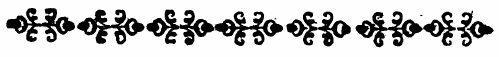
\includegraphics[scale=0.33]{04.aprovacao2.png}
\end{center}
\subsection{Aprovaçaõ.}

\lettrine[findent=2pt, nindent=0pt, lines=2]
{P}{O}r ordem do Padre Alexãdre de Gu\lgS maõ Provinvial de\lgS ta
Provincia do\linebreak Bra\lgS il,
revi o Cateci\lgS mo novamente corrigido
do antigo, que por defeito da impre\lgS -\lgS aõ tinha varios erros,
a\lgSS im na verdade dos vocabulos Bra\lgS ilicos, como nos mofos
com que \lgS e u\lgS a delles no e\lgS tylo de fallar, o que tudo
vay corregido com muita curio\lgS idade, \& diligencia, digno na
verdade de \lgS e imprimir,\& muy nece\lgSS ario para o en\lgS ino
das Aldeas, \& Gentio, que a \lgS eu cargo tem no\lgSS a Companhia,
o que \lgS erá de muito \lgS erviço de Deos, \& o julgo a\lgSS im
por ter intelligencia da me\lgS ma lingoa Bra\lgS ilica. Collegio
do Rio de Janeiro 1. de Junho de 1685.

\begin{center}
    \hspace{60pt}\textit{Lourenço Cardo\lgS o.}
\end{center}
\newpage

\begin{center}
    
\includegraphics[scale=0.33]{05.aprovacao3.png}
\end{center}
\subsection{Aprovaçaõ.}
\vspace*{12pt}

\lettrine[findent=2pt, nindent=0pt, lines=2]
{P}{O}r commi\lgSS aõ do Padre Alexandre de Gu\lgS maõ,
Provincial de\lgS ta Provincia\linebreak
 do Bra\lgS il, revi e\lgS te Cateci\lgS mo 
da Doutrina Chri\lgS -tãa na lingoa Bra\lgS ilica, reformado, \&
emendado, a\lgSS im dos erros da impre\lgSS aõ antiga, como de
muitas diçoẽs, que ou com o tempo perderaõ feu u\lgS o, \& por
i\lgSS o \lgS e igno-ra já hoje, o que \lgS ignificavaõ entaõ,
ou porque pa\lgSS araõ a termos mais cultos, nos quaes tem feito
o u\lgS o, \& a policia a propriedade com que hoje e\lgS taõ
recebidas nos lugares,\& aldeas de\lgS te no\lgSS o Bra\lgS il:
Tambem revi cõ attençaõ a novidade, com que o curio\lgS o ze-lo do
Author \lgS e poz a examinar a variedade das pronunciaçoẽs das
me\lgS mas palavras pa-ra as di\lgS tinguir, nos \lgS entidos,\&
\lgS ignificados; \& para i\lgSS o \lgS ervem as diver\lgS as
pontuaçoẽs,\& plicas, que \lgS obre as dicçoẽs vaõ multiplicadas,
para cuja intelligencia \lgS e póde recorrer\linebreak
a \lgS eu proëmial, onde \lgS e verá com
clare\lgS a, o\linebreak que fem elle pareceria
\lgS uperfluidade, \& conforme ao que entendo ne\lgS ta materia
além de naõ ter cou\lgS a, que encontre a Fé, \& bons co\lgS tumes,
ha de \lgS er e\lgS te livro muito util pa-ra os que \lgS e occupaõ na
doutrina, \& mini\lgS terios das almas entre Indios de\lgS ta lingoa,
\lgS e \lgS e imprimir fielmente \lgS egundo o modo com que vay
di\lgS po\lgS to, porque e\lgS te he hoje o e\lgS tylo da lingoa
commũa, \& u\lgS ual de\lgS tas no\lgSS as partes.

Contém mais e\lgS te livro alguns \lgS upplementos na materia da
admini\lgS traçaõ dos Sacramentos, cou\lgS a na verdade a\lgSS az
nece\lgSS arias para corregir os defeitos que em muitos ca\lgS os
pôdem \lgS ucceder na admini\lgS traçaõ dos actos Sacramentaes:
tudo finalmente digna obra de \lgS eu Author,pois \lgS e parece
tã-to com \lgS eu zelo, \& curio\lgS idade incan\lgS avel, da qual
e\lgS pero \lgS e \lgS iga grande gloria a Deos, \lgS ingular luz
aos operarios de\lgS ta vinha do Senhor, \& notavel proveito a áquelles, em
cuja conver\lgS aõ trabalhamos ne\lgS te Bra\lgS il.
Rio de Janeiro 1.de Junho de 1685.

\begin{center}
    \hspace{60pt}\textit{Simaõ de Oliveira.}
\end{center}
\newpage

\begin{center}
    
\includegraphics[scale=0.33]{06.licencas.png}
\end{center}
\unskip
\vspace*{-20pt}
{\let\clearpage\relax \chapter{LICENÇAS}}
\chaptermark{Licenças.}
\sectionmark{Licenças.}

\lettrine[findent=2pt, nindent=0pt, lines=2]
{O}{}Padre Me\lgS tre Frey Manoel de Sant-\linebreak 
Tiago Qualificador do Santo Offi-\linebreak cio,
ceja o livro de que ne\lgS ta petiçaõ \lgS e faz
mençaõ, \& informe com \lgS eu parecer. Li\lgS boa 18.de Setembro
de 1685.
\unskip
\begin{adjustwidth}{30pt}{0pt}
    \textit{Manoel de Moura Manoel,\\
    Ieronymo Soares.\\
    Ioaõ da Co\lgS ta Pimenta,\\
    O Bi\lgS po Frey Manoel Pereyra,\\
    Bento de Beja de Noronha.}
\end{adjustwidth}

\begin{center}
    Illus\lgS tri\lgSS imo Senhor.
\end{center}

\lettrine[findent=2pt, nindent=0pt, lines=2]
{V}{I} o livro contheudo ne\lgS ta petiçaõ, \& naõ me parece, que
po\lgSS a conter cou-\lgS a que encontre a no\lgSS a Santa Fé, ou
bons co\lgS tumes. S.Franci\lgS co da Cidade em 11. de Outubro de
 1685.

 \begin{center}
    \hspace{60pt}\textit{Fr. Manoel de S.Tiago.}
\end{center}
\newpage

\lettrine[findent=2pt, nindent=0pt, lines=2]
{O}{}Padre Me\lgS tre Fr. Manoel de Santo\linebreak
 Athana\lgS io Qualificador
do Santo Officio veja o livro de que e\lgS ta petiçaõ faz mẽção, \&
informe com o \lgS eu parecer. Lisboa 12. de Outubro de 1685.
\unskip
\begin{adjustwidth}{30pt}{0pt}
    \textit{Manoel de Moura Manoel,\\
    Ieronymo Soares.\\
    Ioaõ da Co\lgS ta Pimenta,\\
    O Bi\lgS po Frey Manoel Pereyra,\\
    Bento de Beja de Noronha.}
\end{adjustwidth}

\begin{center}
    Illus\lgS tri\lgSS imo Senhor.
\end{center}
\vspace*{-4pt}

\lettrine[findent=2pt, nindent=0pt, lines=2]
{P}{O}r mandado de V. Illu\lgS tri\lgSS ima vi o\linebreak
Cateci\lgS mo Bra\lgS ilico, de que e\lgS ta petiçaõ
faz mençaõ. Como o idioma para mim he
peregrino, me pareceo que \lgS ó podia fazer juizo
nas duas lingoas, Portugueza, \& Latina, de que tambem con\lgS ta.
Com tudo, levado da curio\lgS idade, communiquei 
al-\linebreak guns periodos
com Religio\lgS os da minha\linebreak
Provincia, que tinhaõ pa\lgS tado
áquellas partes com a occupaçaõ de mi\lgSS ionarios, \& os
tradu\lgS iraõ em no\lgSS a lingoa com tanta propriedade, que 
de\lgS ejei acharme nos annos da adole\lgS cencia, para a aprender,
\& ali\lgS tarme ne\lgS ta Santa Conqui\lgS ta da conver\lgS ão,
\& \lgS alvação do Gentio, para cujo effeito me pareceo, que o 
pre\lgS ente Cateci\lgS mo naõ \lgS ómente \lgS erá util, mas
preci\lgS amente nece\lgSS ario. Naõ acho nelle cou\lgS que
\lgS eja contra no\lgSS a Fé, ou bons co\lgS tumes. Santo Antonio
dos Capuchos de Lisboa 16. de Outubro de 1685.

\begin{center}
    \hspace{60pt}\textit{Fr. Manoel de S.Athana\lgS io.}
\end{center}

\lettrine[findent=2pt, nindent=0pt, lines=2]
{V}{I}\lgS tas as informaçoẽs, pode\lgS e imprimir o livro de que
ne\lgS ta petiçaõ \lgS e faz mẽçaõ, \& de\lgS pois de
impre\lgSS o tornará para \lgS e conferir,
\& dar licença que corra, \&
\lgS em ella naõ correrá. Lisboa 16. de Outrubo de 1685.
\vspace{\baselineskip}
\begin{adjustwidth}{30pt}{0pt}
    \textit{Manoel de Moura Manoel,\\
    Ieronymo Soares.\\
    Ioaõ da Co\lgS ta Pimenta,\\
    O Bi\lgS po Frey Manoel Pereyra,\\
    Bento de Beja de Noronha.}
\end{adjustwidth}
\vspace{\baselineskip}
\lettrine[findent=2pt, nindent=0pt, lines=2]
{P}{O}de\lgS e imprimir o livro de que a petiçaõ faz menção, \& 
de\lgS pois tornará para \lgS e conferir, \&
dar licença para correr, \& \lgS em ella naõ correrá. Lisboa 23.
de Outubro de 1685.

\begin{center}
    \hspace{60pt}\textit{Serraõ.}
\end{center}

\lettrine[findent=2pt, nindent=0pt, lines=2]
{P}{O}de\lgS e imprimir vi\lgS tas as licenças do Sã-to
Officio, \& Ordinario, \& de\lgS pois de impre\lgSS o tornará a
e\lgS ta Me\lgS a para \lgS e conferir, \& taixar, \& \lgS em 
i\lgSS o naõ correrá.
Lisboa 26. de Outubro de 1685.
\begin{center}
    \hspace{0pt}\textit{Roxas, Lamprea, Marchão, Azevedo,}
\end{center}
\newpage

\begin{center}
    \vspace*{40pt}
    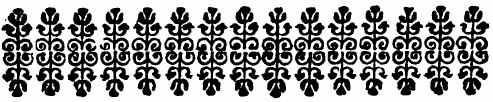
\includegraphics[scale=0.33]{07.erratas.png}
\end{center}
\unskip
\vspace*{-30pt}
{\let\clearpage\relax \chapter{ERRATAS.}}
\chaptermark{}
\sectionmark{}
\lettrine[findent=2pt, nindent=0pt, lines=2]
{P}{A}gina 16. reg. 6. tem Niapykyxoê-\linebreak pemo, lede 
Niapycykixóépemo.\\
Pag. 25. reg. 19. tem agoerabiâra, lede\linebreak ogoerobiâra.\\
Pag. 27. reg. 21. tem ceoroiacegeâbo, lede ceroiacegoâbo.\\
Pag. 49. reg. 8. tem opacatú, lede opacatupe.\\
Pag. 62. reg. 8. tem acepiakine, lede oce-piakine.\\
Pag. 68. reg. 7. tem cetpe catú, lede ceté çupé.\\
Pag. 105. reg. 8. tem oiepiácncá, lede\linebreak oiepiácucá.\\
Pag. 146. reg. 2. tem nhëêugabyagoa-\linebreak
goéra, lede nhëêngabyagoéra.\\
Pag. 155. reg. 14. tem Ipoçang bépe, lede Ipoçangibépe.\\
Pag. 156. reg. 21. tem goemicuagoéra,\linebreak
lede goemicuacugoéra.\\
Pag. 227. reg. 6. tem eremoiecoçúpe, le-\linebreak de
ereimoiecoçúpe.\\
Pag. 247. reg. 6. tem reybâba, lede reymbâba.\\
Pag. 249. reg. ultima. tem onhëâgoâbo, lede enhëãgoâbo.\\
Pag. 315. reg. 21. tem Teomé, lede Teu-\linebreak mé.\\
Pag. 331. reg. 18. \& 333. reg. 7. tem Re-quie\lgS cant, lede 
Requie\lgS cat.
\vspace{\baselineskip}
\begin{center}
    \textit{Além de\lgS tas erratas ha hũas de pouca
    \lgS u\lgS tancia, que por i\lgSS o \lgS enaõ apontaõ.}
\end{center}

\newpage
\vspace*{140pt}
\begin{center}
    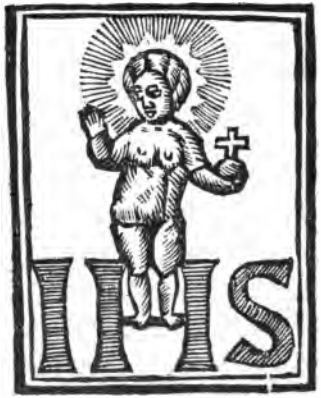
\includegraphics[scale=0.33]{08.jesus.png}
\end{center}
\newpage

\begin{center}
    
\includegraphics[scale=0.36]{09.livro1.png}
    {\large CATECISMO}
    \vspace{5pt}

    {\huge BRASILICO}

    \textit{Da Doutrina Christãa,}
\end{center}
\unskip
\vspace{-30pt}
{\let\clearpage\relax \chapter{\Huge LIVRO I.}}
\unskip
\vspace{-10pt}

\begin{center}
    \textit{Dos primeiros elementos da Fe Chri\lgS tãa,}
\end{center}
\unskip\vspace{-5pt}
\section{Summa dos my\lgS terios, \& \\doutrina Chri\lgS tãa.}

\chaptermark{Summa}
\sectionmark{Da Doutrina Crhi\lgS tãa.}
\unskip\vspace{-5pt}
\par\noindent\rule{\textwidth}{0.4pt}
\unskip\vspace{5pt}
\subsection{Oração do \lgS inal da Cruz.}

%\lettrine[findent =0pt, nindent=0pt, lines=5]
\lettrine[findent =-1pt, nindent=0pt, loversize=-0.1, lraise=0.05, lines=5]
{\zall{S}}{A}NTA Cruz räangâba recé orepy cyrõ iepé, Tupã ore
iár, oré amotarëymbâra çúí. Tû-ba, Täyra, E\lgS pirito Santo
réra pupé. Amen. 
\unskip
\begin{center}
    \unskip
    \textit{Padre No\lgSS o.}
\end{center}
\unskip
\lettrine[findent =4pt, nindent=0pt, lines=2]
{O}{R}é rúb, ybákype tecoár, imöeté pyramo nde réra toicó: Töur
nde Rei-no: Tonhemonhang nderemimotâra yby-pe, ybákype inhemonhânga
iabé: Orérẽ-\linebreak bïú
 âra iabïõ ndoâra eimëeng corí orêbe: Ndenhirõ
oré angaipâba recé orêbe, oré rerecomemoãçâra çupé orénhirõ iabé:
Oremoarucârumé iepé tentaçaõ pupé: Orepy-cyrõ iepé mbäé çüí. Amen.

\subsection{Ave Maria.}
\unskip\vspace*{-12pt}
\lettrine[findent =4pt, nindent=0pt, lines=2]
{A}{V}e Marîa, graça recé tynycémbäé:\linebreak
nde irúnamo iande iâra
recóu: imom-bëú catúpyramo ereicó cunhã çüí; imom-bëú catúpyrabé
ndemembyra JESUS. San-ta Marîa. Tupã cy, etupã monghetá oré 
ïangaipábäe recé cöyr, irã, oré iekyi oré rûmebéno. Amen.

\subsection{Salve Rainha.}

\lettrine[findent =4pt, nindent=0pt, lines=2]
{S}{A}lve Raînha, morauçubâra cy, tecobé, céémbäe, oré
ierobiaçâba, \lgS alve. Ndê-be oroçapucápucai ipëâpyramo Eva 
mem-byramo. Ndébe oronhëangherúr orépöa cémamo, oro iaceguâbo icó
ybytygoâia iaceguâba pupé. Enëĩ ore recé ierureçár\linebreak
ebouĩ nde reçá porauçubâra erobác oré co-ty.
Aë JESUS imombëú catú pyra nde mẽ-byra 
icó iepëaçagoêra cykiré ecepiác ucár, orêbe. Nheranëym,
morauçúb erecoçar\linebreak cëembäé, Virgem Marîa.
Etupã monghetá oré recé,
Santa Marîa Tupã cy, torë angaturâne Chri\lgS to remï-enoĩgoêra
recé oré iecoçubagoâma ri. Amen.

\subsection{Credo.}

\lettrine[findent =2pt, nindent=0pt, lines=2]
{A}{R}obiár Tupã Tûba opácatú mbäe tetiruã monhanga eicatúbä'e,
ybáca, yby abé monhangâra. Arobiár JESUS Chri\lgS to abé Täyra
oiepébäe, acé iâra: E\lgS pirito San-to imonhângâpe pitangamo
onhemonhan-gbäe poêra. Aebäe öár Marîa abábycagoe-rëyma çüí:
Poncio Pilato morobixâbamo cecôreme cerecomémoãbyramo cecóu:\linebreak
ybyrá ioaçâba recé imoiäripyramo cecóu,\linebreak
ijucápyramo, itymimbyramo. Ogoegyb\linebreak
yby apytéripe, âra moçapyra pupé, omanõ-bäe
puêra çüí cecobé iébyri, oieupir ybáky-pe, Tupã Tûba opácatú mbäe
tetiruã monhánga ëicatúbäe, omanõbäe poêra pabẽ\linebreak
recomonhángane. Arobiár E\lgS pirito Santo: Arobiár
Santa Igreja Catholica: Arobiár\linebreak Santos recócatú
ïemoiäó iaöca: Arobiár te-có angaipába recé moroupê Tupã nhirõ:\linebreak
Arobiár acé recobé iebyraõáma: Arobiar\linebreak tecobé opábäeramëyma.
Amen.

\subsection{Artigos da Fé.}

\lettrine[findent =4pt, nindent=0pt, lines=2]
{C}{A}tor\lgS e acéremïerobiarâma.\\ Sete Tupã recé indoâra
nã ëí.

\begin{enumerate}
    \item Arobiar oiepé Tupã opácatú mbäe tetiruã monhânga
    eicatúbäe.
    \item Arobiár túbamo cecó.
    \item Arobiár täyramo cecó.
    \item Arobiár E\lgS irito Santóramo cecó.
    \item Arobiár opacatú mbäe tetiruã monhángáramo cecó.
    \item Arobiár moropycyroánamo cecó.
    \item Arobiár tecobé opábäeramëyma mëéngâramo cecó.
\end{enumerate}
\noindent
Sete JESUS Chri\lgS to ace röó raragoéra rece indoâra nã ëí.
\begin{enumerate}
    \item Arobiár äé Tupã Täyra E\lgS pirito Santo
    i-monhangâpe pitángamo inhemonhangagoéra.
    \item Arobiár Virgem Marîa çüí ïaragoéra, 
    a-babycagoérëymamo cecó pupé memé.
    \item Arobiár acé recé ybyrá ioaçába recé imo-iaripyroéramo,
    ïjucápyroêramo, itymim-byroêramo cecó.
    \item Arobiár yby apytéripe igoegybagoêra, acé rúbypy
    caräíbetá angoéra äépe turâma oçarõbäe renocémagoérabé.
    \item Arobiár âra moçapyra recé cecobé iebyragoéra.
    \item Arobiár ybákype ïieupiragoéra Tupã Tû-ba
    ecatüâba coty cénabé.
    \item Arobiár árapapâne turãgoâma oicobébäe,
    omanõbäepoéra pabẽ recó catúagoéra, cecóangaipgoérabé 
    repymëénga.
\end{enumerate}

\subsection{Mandamentos da Ley de Deos.}

\lettrine[findent =4pt, nindent=0pt, lines=2]
{D}{E}z Tupã acé recómonhangâba.\\
1. Eimöeté oiepé Tupã.
\begin{enumerate}
    \setcounter{enumi}{1}
    \item Anheté erétenhëumé Tupã rêra renõia.
    \item Eimöeté Domingo, âra marã teco abëymabé.
    \item Eimöeté nde rûba, nde cy abé.
    \item Eporapitíümé.
    \item Eporopotarumé.
    \item Emondarõumé
    \item Nde remöémumé abá recé.
    \item Enhemomotárumé nde rapixára remire-có recé.
    \item Enemomotárumé abá mbäe recé.
\end{enumerate}

\noindent Nã ëíbäe pupé pabé aipóbäe rûi.
\begin{enumerate}
    \item Opácatú mbäe tetiruã acé çauçûba çoçé acé Tupã
    rauçûba.
    \item Oieauçûba iábé acé öapixâra rauçûbanó.
\end{enumerate}

\subsection{Mandamentos da Santa Madre Igreja.}

\lettrine[findent =2pt, nindent=0pt, lines=2]
{S}{I}nco Santa Madre Igreja acé recómo-\linebreak nhángâba.
\begin{enumerate}
    \item Domingo recé âra marátecoabëyma recébé Mi\lgSS a 
    rendûba.
    \item Ceixú ïabiõ nhemombëú.
    \item Pa\lgS coa iabiõ Tupã âra.
    \item Santa Madre Igreja iecüacúpoâia 
    iabiõ iecuacûba.
    \item Opácombó iabiõ Tupã çupé oiepé acémbäe moiaóca:
    oemitymbuérypy pupé Tupã potámëéngano.
\end{enumerate}

\subsection{Sacramentos.}
\begin{center}
     \textit{Sete Santa Madre Igreja Sacramentos.}
\end{center}
\comecalista{1.}{2.}{Y}{C}
    {aräîba pupé nhemboiaçûca.\\
    Acé cybápe abaré guaçu nhandy\\\hspace*{14pt} caräíba nonga.}
\begin{enumerate}
    \setcounter{enumi}{2}
    \item Tupã râra.
    \item Nhemombëú.
    \item Acé rëõ ianondé nhandy caräîba râra.
    \item Nhemöabaré.
    \item Mendâra.
\end{enumerate}
\vspace{\baselineskip}

\subsection{Peccados Capitaes.}

\lettrine[findent =2pt, nindent=0pt, lines=2]
{S}{e}te opácatú angaipâba nhemonhángáb ypy.
\begin{enumerate}
    \item Morerobiarëyma.
    \item Tecatëyma.
    \item Moropotâra.
    \item Nhemoyrõ.
    \item Mbäé u, memé cäú eté eté.
    \item Abá mbäé catú möacy.
    \item Tupã recó recé nhemboryryi ëyma.
\end{enumerate}

\subsection{Virtudes contra os \lgS ete peccados.}
\begin{center}
    Sete tecó catu aipó tecó angaipâba robaixoára nã ëí.  
\end{center}
\comecalista{1.}{}{M}{O}
    {rerobiarëyma robaixoâra\\\hspace*{10pt} Nhemöeté ëyma.}
\begin{enumerate}
    \setcounter{enumi}{1}
    \item Tecateyma robaixoára\\\hspace*{40pt} Tecatëyma.
    \item Moropotâra robaixoára\\\hspace*{40pt} Moropotarëyma.
    \item Nhemoyrõ robaixoára\\\hspace*{40pt} Toçânga.
    \item Mbäéu eté, cäú etébé robaixoára\\
    \hspace*{40pt} Oiá nhóte mbäëú, memé cäú.
    \item Abá mbäé catú möacy robaixoára\\\hspace*{40pt}
    Joauçûba.
    \item Tupã recó recé nhemboryryiëyma robaixoâra. Tupã
    recó recé nhemboryryia.
\end{enumerate}

\subsection{Obras de mi\lgS ericordia.}
\begin{center}
    Cator\lgS e acé abá rauçubpa çâba.\\
    Sete abá reté recé ndoâra nã ëí.
\end{center}
\comecalista{1.}{2.}{A}{M}
    {byacybôra póia.\\Uceibôra moyú.}
\begin{enumerate}
    \setcounter{enumi}{2}
    \item Icatupendoâra moäôba.
    \item Mbäéacybôra repiâca.
    \item Atâra mombytá.
    \item Imomĩauçubipyra renocêma.
    \item Tëõboêra tyma.
\end{enumerate}

\noindent Sete abá anga recé ndoâra nã ëí.
\begin{enumerate}
    \item Abá çupé recócatúçagoâma mombëú.
    \item Itecócüabëymbäe motecocüâba.
    \item Oicote bẽbae möapycyca.
    \item Oicomemoãbäe renonhêna.
    \item Oguerecomemoãçâra çupé nhirõ.
    \item Abá marã cecó agoérĩ recé nheranëy-\linebreak ma.
    \item Oicobébäe recé omanõbäepoéra recé bé Tupã monghetá.
\end{enumerate}

\subsection{Bemaventuranças.}
\begin{center}
    Oito tecó catu eté rerecoáramo Oporomöĩgobêbäe.    
\end{center}
\unskip
\comecalista{1.}{}{T}{E}
    {có catú eté rerecoâra, öemimotáriboé imbäé ëymbäe,
    imbäéramo ybâca recóune.}
\begin{enumerate}
    \setcounter{enumi}{1}
    \item Tecó catú eté rerecoâra, onheranëymbäe, Aëbäe
    yby oguerecóune.
    \item Tecó catú eté rerecoâra, oiaceõbäe, Aé-bäe
    imöapycykipyramo cecóune.
    \item Tecó catú eté rerecoâra, tecó catú uceitâra
    Aébäe imoytarõbyramo cecóune.
    \item Tecó catú eté rerecoâra, iporaububári-\linebreak bäe,
    Aébäe çauçubâri pyramo cecóune. 
    \item Tecó catú eté rerecoâra, ipyámemoãëy-mbäe,
    Aébäe Tupã ocepiakine.
    \item Tecó catú eté rerecoâra, oporomonhyrõbäe,
    Aébäe Tupã räyri iábamo cecóune.
    \item Tecó catú eté rerecoâra, tecó catú recé
    mbäé poraráçâra, Aébäe ombäéamo ybâ-ca rerecóune.
\end{enumerate}

\subsection{Doẽs do E\lgS pirito Santo.}
\unskip
\vspace*{-2pt}
\begin{center}
    Sete Tupã E\lgS pirito Santo remimëênga.
\end{center}
\unskip
\comecalista{1.}{2.}{T}{U}
    {pã rermimotâra rupí mbäé cüâ-pa. Tecocüâba.}
\begin{enumerate}
    \setcounter{enumi}{2}
    \item Tupã omotecocüâba rupí mbäé mõmbëú.
    \item Myatã.
    \item Mbäécüâba.
    \item Morauçubâra.
    \item Tupã möabá eté.
\end{enumerate}

\subsection{Virtudes Theologaes.}

\begin{center}
    Moçapyr tecó catú Tupã mombegoâba.
\end{center}
\comecalista{1.}{2.}{T}{U}
    {pãrerobiâra.\\Tupã recé ierobiâra}
\begin{enumerate}
    \setcounter{enumi}{2}
    \item Tupã rauçûba
\end{enumerate}

\subsection{Virtudes Cardeaes.}

\begin{center}
    Quatro tecó catú itá.
\end{center}
\comecalista{1.}{2.}{T}{E}
    {có râma ri iepyçacá.\\Abá çupé imbäé mëenga.}
\begin{enumerate}
    \setcounter{enumi}{2}
    \item Myatã.
    \item Mbäé äíba potâra renonhêna.
\end{enumerate}

\subsection{Potenciais da Alma.}

\begin{center}
    Mopyr, mbäé recé acé anga ecatüâba.
\end{center}
\comecalista{1.}{2.}{M}{B}
    {äé recé imäendüaçâba.\\Itecócüâba.}
\vspace{2pt}
\begin{enumerate}
    \setcounter{enumi}{2}
    \item Imbäe potaçâba.
\end{enumerate}

\subsection{Sentidos Corporaes.}
\begin{center}
    Cinco acé mbäé cüapába.
\end{center}
\comecalista{1.}{2.}{M}{A}
    {ẽ\\Mbäé rendúba.}
\vspace{2pt}
\begin{enumerate}
    \setcounter{enumi}{2}
    \item Mbäé retûna.
    \item Mbäé ïupyra räanga.
    \item Mbäé recé mocôca andûba.
\end{enumerate}

\subsection{Novi\lgSS imos.}
\begin{center}
    Quatro abárecó mondycâba.    
\end{center}
\comecalista{1.}{2.}{T}{E}{õ.\\Tupã acé recó cüapâba.}
\begin{enumerate}
    \setcounter{enumi}{2}    
    \item Anhaga ratá.
    \item Ybákype toryba.
\end{enumerate}
\unskip
\vspace{6pt}%\baselineskip}
\subsection{Acto de Contrição.}
\unskip\vspace*{-0.7\baselineskip}
\begin{center}
    Angaipâba möacypâba.
\end{center}
\unskip
\vspace{\baselineskip}
\lettrine[findent =2pt, nindent=0pt, lines=2]
{X}{E}rubiguy Tupã eté, opácatú mbäé çauçubipyra çocé nde
rauçupâpe, icó nde angaturámeté opácatú mbäé iangaturám-bäe
çocé nde recó cüâpa, xe pyápe catú aimö-acy nde nhëenga
abyagoéra, aroirõ opácatû tecó angaipâba, ceroieby potarëyma.
Nde nhirõ tené xêbo, xe iâra JESUS Chri\lgS to ruguy, xe 
anga repymondycâba recé: cecé é guiierobiâbo nde nhirõ recé
taiecoçúb coytene. Amen.

\subsection{Confi\lgSS aõ géral.}

\lettrine[findent =2pt, nindent=0pt, lines=2]
{A}{N}he mombëû Tupã opacatú mbäe tetiruã monhânga ëicatúbäe
çupé, Santa Maria ababycagoerëyma çupébé, S. Miguel Caräíbebé,
Saõ Joaõ Bauti\lgS ta çupebé, Santos Apo\lgS tolos Saõ Pedro,
Saõ Paulo çupébé, opacatpu Santos çupébé, ndêbo bé, Päí aba-ré,
cetanhé xe angaipagoéra recé, tecó angaipába ri xe mäendüáramo,
xe nhëengaíbamo guitecómemoâmo, xe angaipábetéramo. Emonãnamo
aieruré Santa Maria a-babycagoerëyma çupé, Saõ Miguel Caräíbebé,
çupébé, Saõ Joaõ Bauti\lgS ta çupebé, Santos Apo\lgS tolos
Saõ Pedro, Saõ Paulo çupébé, opácatú Santos çupébé, ndêbo bé,
Päí Aba-ré, ipabé xe recé pe tupã Monghtá râma ri.

%Livro 2
\newpage
%\vspace*{150pt}
\begin{center}
    \vspace*{20pt}
    
\includegraphics[scale=0.33]{10.livro2.png}
\end{center}
\unskip
\vspace{-30pt}
{\let\clearpage\relax \chapter{\Huge LIVRO II.}}
\unskip
\vspace{-2pt}
\begin{center}
    {\large CATECISMO}
\end{center}
\unskip
\begin{center}
    Do \lgS inal da Cruz, nome de Chri\lgS taõ,\\
    \& Invocaçaõ dos Santos.\\
    \vspace{6pt}\textit{Com a Explicaçaõ do Padre No\lgSS o,\\
    \& Ave Maria.}
\end{center}
\unskip
\par\noindent\rule{\textwidth}{0.4pt}
\unskip\vspace{-3pt}
\section{DIALOGO I.}
\unskip\vspace{-3pt}
\subsection{Do \lgS inal da Santa Cruz.}

\chaptermark{Dialogo I.}
\sectionmark{do \lgS inal da Cruz.}

\hspace{-10pt}
\begin{minipage}[t]{0.16\linewidth}
    Me\lgS tre.\\ \\Di\lgS cip.\\Me\lgS tre.\\ Di\lgS cip.
\end{minipage}
\begin{minipage}[t]{0.95\linewidth}
    \lettrine
    [findent =-2pt, nindent=0pt, loversize=-0.2, lraise=0.05, lines=5]
    {\zall{M}}{B}äépe Chri\lgS taõs iecüapâba?\\
    Santa Cruz.\\
    Maránamope?\\
    Iárybo omanõmo iandé iâra iandé repymëengagoéra recé,
    anhan-\linebreak ga ratá çüí iandé pycyrõ recebé.
\end{minipage}\\

\begin{alternate}
    \item Marã ḯpe acé oiobaçâba?
    \item Santa Cruz räangâba recé orepycyrõ ie-pé,
    Tupã oréiar, oré amotarëymbâra\linebreak
    çüí: Tuba, Täyra, E\lgS pirito Santo rêra\linebreak
    pupé. Amen, ëí.
    \item Maránamopé acé ocybápe iobaçâba möí-ni?
    \item Táxepycyrõ Tupã maenduaçâba äíba çüí oiâbo.
    \item Manránamopé acé oiurúpe çäánghino?
    \item Toipëá Tupã nhëéngmemoã xe iurú çüí oiâbo.
    \item Maránamopé acé opotïápe imöíni?
    \item Táxepëá Tupã tecó angaipâba çüí acé\linebreak
    nhyã çüí ocembäe, oiâbo.
    \item Maránamobé pé acé iobaçâbi?
    \item Santi\lgSS ima Trindade, Tûba, Täyra, E\lgS pirito
    Santo, Moçapyr abá, oiepé Tubã mombeguâbo nhé.
    \item Bäéreme tépé acé iobaçábine?
    \item Mbäé ypyrûnga iabiõ, coêpe marã tecó omöanghecoâime.
    \item Bäéremebépe?
    \item Okér ianondé, opâcagoéripe, ôca çüí o-cémabé.
    \item Oçobacápe acé oemïurâma?
    \item Oçobacáb.
    \item Maránamopé?
    \item Táxemarã ume igoâbo, oiâbo.
    \item Maránamopé acé iobaçáb etá etáone?
    \item Táxepycyrõ Tupã xe çumarã çüí coépe marã xerecoápe, oiâbo.
    \item Abá pe acé çumarã?
    \item Anhânga.
    \item oierokype acé Cruz çupé?
    \item Oieroky.
    \item Marã, ybyrá çupé nhépe, acé ierokyu?
    \item Näani, çaangabijára çupéé, cecé omäen-düáramo.
    \item Abápe Cruz räangâbiâra?
    \item Iandé iâra JESUS Chri\lgS to.
    \item Maránamo pé?
    \item Cecé imboiaripyramo omanômo oie-\linebreak 
    möatã agoéra recé.
    \item Oierokype acé iandé iâra räangâba çu-pé, Santa Maria
    Tupã cy räangâba çupé, Santos ybakypendoára räangâba çupébé?
    \item Oieroky.
    \item Ybákype oicóbäe möeté iabé pe acé çä-angâba möetéo?
    \item Iiabé.
    \item Marã, itánhépe coipó ybyrá, nhäûma çüí imonhanghimbyra
    nhé pe acé oimoeté?
    \item Näâni, çäangabijâra é: çäangábamo cecó reme, cecé
    omäendüáramo.
\end{alternate}

\par\noindent\rule{\textwidth}{0.4pt}
\unskip\vspace{5pt}
\section{DIALOGO II.}
\unskip\vspace{-3pt}
\subsection{Do Nome de Chri\lgS taõ.}

\chaptermark{Dialogo II.}
\sectionmark{do Nome de Chri\lgS taõ.}

\comecalista{M.}{}{M}{A}{rápe imongaräíbipyra renõidábeté?}
\vspace{4pt}
\begin{altereven}
    \item Chri\lgS taõs.
    \item Maránamopé?
    \item Chri\lgS to iande iâra rerobiaçáramo cecóreme, cecó
    mombeguáramo cecóreme.
    \item Niapycykixóépemo cerobiaçâra opyápe nhóte cerobiâbo?
    \item Niapycykixóemo, omanõmo tiruá cerobiámo.
    \item Iandé iâra JESUS Chri\lgS to çüí.
    \item Abápe JESUS Chri\lgS to?
    \item Tupã eté, apŷabeté iandé iabêbé.
    \item Manránamopé acé Tupã eté, ïeú ixupé?
    \item Tupã Tûba räyreté oiepêbäêramo cecóreme.
    \item Aêpe marã apyábetêramo cecóu iandê-iabê?
    \item Cunhã angaturâma ababycagoerëyma\linebreak
    Santa Maria Ceríbäe membyramo cecó\linebreak reme.
    \item Nixyítepe Tupã etéramo oicôbo?
    \item Nixui, nacetéi, nïypyi Tupã etéramo oi-côbo.
    \item Natûbi tépé apyábetéramo oicôbo?
    \item Na tûbi, onhemonhanghé ocy iatoĩby-rëyma righépe.
\end{altereven}

\vspace{3pt}
\par\noindent\rule{\textwidth}{0.4pt}
\unskip\vspace{5pt}
\section{DIALOGO III.}
\unskip\vspace{-3pt}
\subsection{Do \lgS anti\lgSS imo Nome de Je\lgS us, \&
            invocaçaõ dos Santos.}

\chaptermark{Dialogo III.}
\sectionmark{da invocaçaõ dos Santos.}

\comecalista{M.}{D.}{A}{B}
    {ápe acé ocenoĩ oicótebêmo?\\
    JESUS ocenoĩ.}
\begin{alternate}
    \item Maránamopé?
    \item Táxe pycyrõ marã tecó çüí, oiábo.
    \item Marã oiâbo pé acé JESUS ïeú?
    \item Moropycyrõâna oiâbo.
    \item Oierokype acé JESUS éreme?
    \item Oierokype.
    \item Marã éreme bépé acé ierokyo?
    \item Santa Maria éreme.
    \item Maránamopé?
    \item Tupã cyramo cecóreme nhé.
    \item Abá çupéé acé ierúréo öeté maranëyma-õâma recé,
    öanga recocaturâma recébé?
    \item Tupẽ çupé.
\end{alternate}
\begin{alternate}[parsep=-5.4pt]
    \item Abápe acé recé Tupã manghetaçáramo cecóu?
    \item Santa Maria Tupã cy, Caräíbebé aceraroâna abé.
    \item Acerarõánamo tepé Caräíbebé recóu?
    \item Acerarõánamo.
    \item Oiabiõpé acé cerecóu?
    \item Oiabiõ.
    \item Mbäérâma recépe Tupã imëenghi acébé?
    \item Acé çumarã çüí acé rarõ agoâma recé.
    \item Mbäé, mbäé çüípe acerarõu?
    \item Anhánga çüí, tecó angaipâba çüí, mbäé äíba çüí bé.
    \item Marã ëípe acé caräíbebé öaroâna mon-ghetâbo?
    \item Caräíbebé xe rarõâna, xe pëá iepé mbäé äíba çüí
    cori, Tupã remimotâra rupí xe\linebreak moĩgôbo, ëí.
    \item Abá, abápe acé recé Tupã monghetaçáramo cecóu?
    \item Santos etá ybákype tecoâra.
    \item Emonánamo pé acé ieruréo Santos etá çupé.
    \item Emonánamo, memé ogueriiâra çupé.
    \item Marã ëípe acé ixupe oierurêbo?
    \item Peimonghetá Tupã iandé iâra ixêbo, taxerauçubár ëí.
\end{alternate}
\begin{alternate}[leftmargin=8pt]
    \item Mbäé mbäéremepé acé ieruréo ixupé?
    \item Iepínhé, memé ïâra áreme no.
    \item Maránamope acé Sãtos âra cüabi, imöetêbo, ipupé
    toryba monhânga?
    \item Ybákype Tupã imöeté catú recé omäen-düáramo.
    \item Maránamo bépé?
    \item Cecó catúgoêra rupi oicó potá taicó catúïiabébé
    cá oiâbo.
    \item Maránamobépé?
    \item Çauçûpa, totupãmonghetá xe recé ixe
    oguauçûme,oiâbo,ixe omöetéreme oiâbo.
    \item Mbäerama rí bépe acé Santos âra cüâbi?
    \item Tupã ixupé tecó catú mëengâra möeté agoâma recé.
    \item Marãngatúpe acé recóu Tupã ókype oikeâbo?
    \item Oieypyi y caräíba pupé.
    \item Mbäé râma recépé?
    \item Anhânga monhegoacemãõâma recé.
    \item Mbäé râma recébépe?
    \item Acé angaipá mirĩ recé, acêbo Tupã nhi-rõ aõgoâma recé.
    \item Marãgatúpe acé recóu ipipé oieypyia?
    \item Oimöacy catú öangaipâba opyápe.
    \item Marã ëípe acé Tupã okype oikeâbo, y caräíba pupé 
    oieyoyîa? 
    \item Y imongaräíbipyra toicó xe anga 
    recobéçáramo, tomonhegoacémucár anhân-ga xe çüí. Amen 
    Je\lgS us, ëí.
    \item Ocypyibépe acé tyby y caräíba pupé?
    \item Ocypyi bé.
    \item Mbäérâma recépe?
    \item Tonhegoacém anhânga ixüí, oiâbo.
    \item Marã ëípe acé oké ianondé, Tupã mon-ghetâbo.
    \item Xe iár JESUS Chri\lgS to, nde réra pupé a-nhenõg
    guiképotá, äé taxerobaçáb, äé taxerarõ, äé abé taxepycyrõ,
    äe abé taxereraçó ogorypápe, ëí.
    \item Marã ëípe acé opâca roire?
    \item Xe iár JESUS Chri\lgS to eceçapé corí xe\linebreak
    anga reçá, taiabyuméné icó âra pupé nde nhëênga,
    nde remimotâra rupí catú xe\linebreak moingó iepé corí, ëí.
\end{alternate}

\vspace{2pt}
\par\noindent\rule{\textwidth}{0.4pt}
\unskip\vspace*{-4pt}
\section{DIALOGO IV.}
\unskip\vspace{-3pt}
\subsection{Do Padre No\lgSS o.}

\chaptermark{Dialogo IV.}
\sectionmark{Do Padre No\lgSS o.}
\vspace*{-6pt}
\comecalista{M.}{D.}{M}{A}
    {rã ëípe acé Tupã monghetâbo?\\
    Oré rúb, ybákype tecoár, ëí.}
\begin{alternate}
    \item Abápe aipóbäé oimonháng erímbäé 
    çä-anghypyâbo?
    \item Iandé iâra JESUS Chri\lgS to äé oçäang\linebreak
    erímbäé oiurú rupí catú.
    \item Mbäérâma recépe?
    \item Tupã monghetá recé iandé mböébo nhé.
    \item Onhemoçainân pabẽpe Chri\lgS taõs aipó-bäé
    cüabaõáma recé?
    \item Ouhemoçainân pabẽ.
    \item Tupã çupéé acé orerúb ïéu?
    \item Tupã çupé.
    \item Marãpe acé rubamo cecóu?
    \item Acé monhangaretéramo oicôbo.
    \item Marãpe acé monhânghi?
    \item Nã mbäé rüã oimonháng acé angamo,
    onhëênga pupé é imonhânghi.
    \item Nace rûba rüã tepé acé reté oimonháng?
    \item Acé rûba oimonháng bïã, Tupã imo-\linebreak
    nhânga potaçâpe é.
    \item Marã oicôbo bépe Tupã acé rúbamo cecóu?
    \item Acé rûba, acé cy, acé rauçûba çocé, acé rauçûpa,
    öäyretêramo acé rerecôbo.
    \item Marã ëípe acé opyápe Tupã çupé, orerúb, oiâbo?
    \item Taimöeté catú xe rûba cá, taçauçub ca-tú,
    taçapiar catú cá, oiâbo.
    \item Otĩ nhémo cerã iangaipábäé, oré rúb,\linebreak oiâbo
    Tupã çupé?
    \item Otĩ nhémó anhé, otecocüábamo emó.
    \item Marãnamo pe?
    \item Naçapiár icó xerúbeté, oiâbo, naiár icó
    cecó angaturâma, oiâbo.
    \item Marã ëíbépé acé opyápe, oré rúb, oiâbo Tupã çupé.
    \item Arobiár catú ce rûba Tupã recé, ëí: äé xererecó,
    äé xepycyrõ, äé xerecotebẽçâba oimëéng ixêbonê, ëí.
    \item Oierobiácatúpe acé Tupã recé aipó oiâ-bo?
    \item Oierobiácatú, abábiã é öäyra oguerecó catú,
    memétipó Tupã mbäé tetiruã iára-mo oicóbäé acé rauçubáne,
    oiâbo.
    \item Marãnamo pé acé orérúb ïeú, Xerûb öénhóteëyma?
    \item Oioanametéramo pabẽ, Tupã räyretéra-mo pabẽ cecó
    cüâpa, oiöauçûba potá.
\end{alternate}

\subsection{Que e\lgS tàs nos Ceos.}
\unskip\vspace*{-0.7\baselineskip}
\comecalista{M.}{D.}{M}{A}
    {mópe Tupã recóu?\\
    Ybákype, ybype, opacatú mbäé\linebreak mopôri.}
\begin{alternate}
    \item Maránamo tépé, ybákype tecóar, acé ïeú ixupe?
    \item Ybakype é iangaturambäé çupé iepiacu-cá potéreme.
    \item Maránamobépé.
    \item Ybákype é ogubeté, öemimotáreté recó-cüâpa, acé
    Tupã repiacäûbi, yby árybo\linebreak ocoábäé reroyrómo.
    \item Marã ëípe acé opyápe ybâca recé omäêmoné?
    \item Ybákype é Tupã xe rubeté recóu mã ëí-né, açó
    temo xe rûba pyri, xe retametépe mã, ëíné.
    \item Naceretâma rüãtepé icó yby acé recoâ-ba?
    \item Näani, ybâca porâma recé é Tupã acé\linebreak
    monhânghi: atáramo é acé recóu icó yby pupé.
\end{alternate}
\unskip\vspace*{-0.7\baselineskip}
\subsection{Santificado \lgS eja o teu Nome.}
\unskip\vspace*{-0.7\baselineskip}
\comecalista{M.}{}{M}{B}
    {oby mbäé recé pe acé ierureó,\\
    \hspace*{10pt}orérúb ëíbäé räânga?}
\begin{altereven}
    \item Sete mbaé recé.
    \item Marã ëípe ïypy?
    \item Imöeté pyramo nde rêra toicó, ëí.
    \item Marã oiâbo  pé acé aipó ïéu Tupã çupé?
    \item Tandererobiá pabẽ abá, ogúbamo, omo-nhangáramo
    nde recó cüâpa, nde möetê-bo, oiâbo.
    \item Abá abápe Tupã réra oimöeté ucár?
    \item Chri\lgS taõs inhëênga rupí tecoâra.
    \item Marã iabépe?
    \item Chri\lgS taõs recó catú repiâca é ipó, 
    imongarâibipyrëyma Tupã mombëú catú, ce-có recé 
    onhe momotá.
    \item Aëpe Chri\lgS taõs Tupã nhëêngabyâra,\linebreak
    marã? 
    \item Aë ipó Tupã noimöangaturâmi imonga-räíbipyrëyma
    çupé, cecó potárucáreyma.
\end{altereven}

\subsection{Venha a nós o teu Reino.}

\comecalista{M.}{D.}{M}{A}
    {rã ëípe amó äé acé ierureçâba?\\
    Tour nde Reino, ëí.}
\begin{alternate}
    \item Marã oiâbo pé acé aipó ïeú?
    \item Nde nhõ tore recó iepé, oré rubixácatúramo
    eicôbo, oiâbo.
    \item Marã oecó potápe acé aipó ïéu?
    \item Tupã boiáramo nhõ oicópotá, inhëên-ga rapiá potá,
    anhânga oiáramo cecó potarëyma.
    \item Marã oicôbo tepé acé anhânga rembï-\linebreak auçúbamo
    cecóu?
    \item Öangaipábamo, Tupã nhëênga abyâbo.
    \item Marã oiâbo bépe acé, Töúr nde Reino, ïéu?
    \item Toroguacém te ybákype nde recóabetê-pe, nde
    iepuacucáçápe, oiâbo.
    \item Mbäé pe Tupã oimëéng acêbe ybákype ne?
    \item Tecobé opabäéramëyma.
    \item Erimbäé pe né?
    \item Acé rëõ riré ybákype acé ânga reraçôbo.
    \item Aëpe acé reté rëombuêra marã?
    \item Arapábiré imöingobéiebyri opyri cera-\linebreak çôbo
    auieramanhé ne
\end{alternate}

\subsection{Seja feita a tua vontade, \&c.}

\comecalista{M.}{D.}{M}{A}
    {rã ëípe amó äé.\\
    Tonhemonhang nde remomotâra ybype
    ybákype inhemonhang iabé, ëí.}
\begin{alternate}
    \item Marã oiâbope acé aipó ïéu?
    \item Toicó pabẽ ybypeçoâra nde remimotâra
    rupí ybakygoâra recó iabé oiâbo.
    \item Noimomarã mirĩ angâipe ybakygoâra\linebreak
    Tupã remimotára?
    \item Näanagai: acé iangaipábäé ipó icó yby pé Tupã
    remimotâra noimonhânghi.
    \item Marãngatúpé Tupẽ acé recó oipotar?
    \item Oipotár acé agoerabiâra, öauçûba, öecö-abyëyma.
    \item Marãnamobépe acé tonhemonháng nde remimotára,
    ïéu Tupã çupé?
    \item Mbäé poxy ogoeté remimotâra rupi oicópotarëyma;
    anhânga remimotâra morãbué potábé no.
    \item Mbäé mbäépe anhânga oipotár?
    \item Acé Tupã nhëênga aby, öatápe acé rera-çó potá;
    ybákype Tupã rorypápe iandé çó potarëyma.
\end{alternate}

\subsection{O paõ no\lgSS o de cada dia, \&c.}

\comecalista{M.}{D.}{M}{A}
    {rã ëípe amó äé acé ieruréçâba?\\
    Oré rembïú âra iabiõdoâra eimë-éng cori orebê, ëí.}



\end{document}